% !TeX program = pdflatex
\documentclass[border=6pt]{standalone}
\usepackage{tikz}
\usetikzlibrary{arrows.meta, positioning, calc}

\definecolor{MediumRed}{rgb}{0.925, 0.345, 0.345}
\definecolor{MediumGreen}{rgb}{0.37, 0.7, 0.66}
\definecolor{MediumBlue}{rgb}{0.015, 0.315, 0.45}
\definecolor{DarkBlue}{rgb}{0.05, 0.15, 0.35}

\def\s{0.30}

\begin{document}
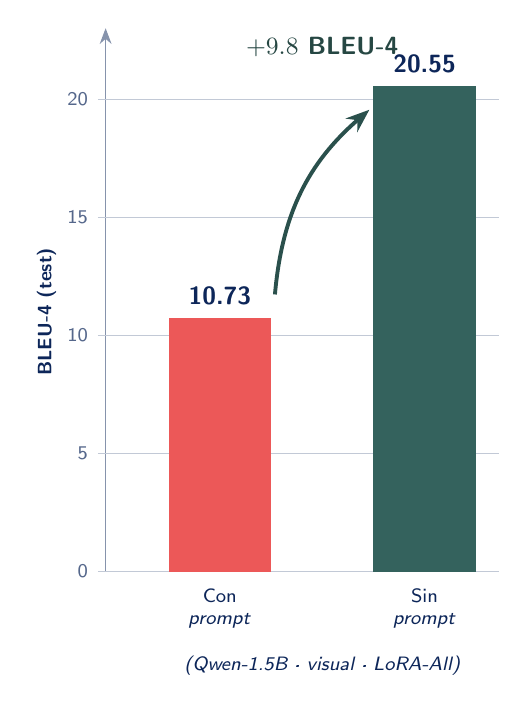
\begin{tikzpicture}[font=\sffamily]

% eje
\draw[DarkBlue!50, -{Stealth[length=2mm]}] (-0.4,0) -- (-0.4,{23*\s});
\foreach \y in {0,5,10,15,20}{
    \draw[DarkBlue!25] (-0.5,{\y*\s}) -- (4.6,{\y*\s});
    \node[font=\sffamily\scriptsize, text=DarkBlue!70, anchor=east] at (-0.5,{\y*\s}) {\y};
}
\node[font=\sffamily\scriptsize\bfseries, text=DarkBlue, rotate=90] at (-1.15,{11*\s}) {BLEU-4 (test)};

% barras
\fill[MediumRed] (0.4,0) rectangle (1.7,{10.73*\s});
\node[font=\sffamily\small\bfseries, text=DarkBlue, anchor=south] at (1.05,{10.73*\s+0.05}) {10.73};
\node[font=\sffamily\scriptsize, text=DarkBlue, anchor=north, align=center] at (1.05,-0.1)
    {Con\\\textit{prompt}};

\fill[MediumGreen!55!black] (3.0,0) rectangle (4.3,{20.55*\s});
\node[font=\sffamily\small\bfseries, text=DarkBlue, anchor=south] at (3.65,{20.55*\s+0.05}) {20.55};
\node[font=\sffamily\scriptsize, text=DarkBlue, anchor=north, align=center] at (3.65,-0.1)
    {Sin\\\textit{prompt}};

% flecha de mejora
\draw[-{Stealth[length=3mm]}, MediumGreen!45!black, line width=1.4pt]
    (1.75,{10.73*\s+0.3}) to[bend left=22] (2.95,{20.55*\s-0.3});
\node[font=\sffamily\small\bfseries, text=MediumGreen!40!black] at (2.35,{20.55*\s+0.5})
    {$+9.8$ BLEU-4};

\node[font=\sffamily\scriptsize\itshape, text=DarkBlue, align=center, anchor=north] at (2.35,-0.95)
    {(Qwen-1.5B · visual · LoRA-All)};

\end{tikzpicture}
\end{document}
